\section{Análise sintática {\it top-down}}

\begin{frame}[fragile]{Análise sintática recursiva-descendente}

    \begin{itemize}
        \item A análise sintática \textit{top-down} pode ser interpretada como uma tentativa de se encontrar uma derivação mais à esquerda para uma cadeia da
            entrada
       %\pause

        \item Outra forma de interpretar esta análise é como uma tentativa de construção de uma árvore gramatical a partir da raiz, criando os nós da árvore
            em pré-ordem
       %\pause

        \item No caso geral, a análise sintática recursiva-descendente pode envolver algum nível de retrocesso
       %\pause

        \item Um caso especial da análise sintática recursiva-descente é o dos analisadores preditivos, que não demandam retrocesso
    \end{itemize}

\end{frame}

\begin{frame}[fragile]{Retrocesso}

    \begin{itemize}
        \item Certas gramaticas impõem ao analisador recursivo-descendente a necessidade de um retrocesso na análise
       %\pause

        \item Por exemplo, considere a entrada $w = cad$ e a gramática
        \[
            \begin{array}{l}
                S \to cAd \\
                A \to ab\ |\ a
            \end{array}
        \]
       %\pause

        \item A análise inicia construindo a raiz da árvore sintática, rotulada como $S$
       %\pause

        \item Ao ler o primeiro símbolo da entrada, o caractere $c$, o analisador expande a produção de $S$ para gerar os filhos e obter
        \begin{center}
            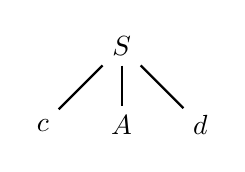
\begin{tikzpicture}
                \node (A) at (6, 6) { $S$ };
                \node (B1) at (5, 5) { $c$ };
                \node (B2) at (6, 5) { $A$ };
                \node (B3) at (7, 5) { $d$ };

                \draw[thick] (A) to (B1);
                \draw[thick] (A) to (B2);
                \draw[thick] (A) to (B3);
            \end{tikzpicture}
        \end{center}
        
    \end{itemize}

\end{frame}

\begin{frame}[fragile]{Retrocesso}

    \begin{itemize}
        \item O filho mais à esquerda reconhece o caractere $c$, de modo que o apontado avança para o segundo símbolo da entrada, o caractere $a$
       %\pause

        \item A análise usa a primeira alternativa das produções-$A$ para obter
        \begin{center}
            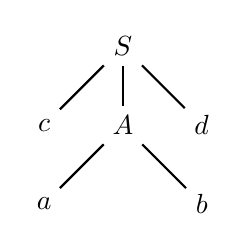
\begin{tikzpicture}
                \node (A) at (6, 6) { $S$ };
                \node (B1) at (5, 5) { $c$ };
                \node (B2) at (6, 5) { $A$ };
                \node (B3) at (7, 5) { $d$ };
                \node (C1) at (5, 4) { $a$ };
                \node (C2) at (7, 4) { $b$ };

                \draw[thick] (A) to (B1);
                \draw[thick] (A) to (B2);
                \draw[thick] (A) to (B3);
                \draw[thick] (B2) to (C1);
                \draw[thick] (B2) to (C2);
            \end{tikzpicture}
        \end{center}
       %\pause

        \item A folha à esquerda reconhece o caractere $a$, mas a folha à direita, rotulada $b$, não reconhece o caractere $d$
       %\pause

        \item Aqui acontece o retrocesso: os filhos são descartados e, ao retornar ao nó $A$, é usada a segunda alternativa das produções-$A$ 
    \end{itemize}

\end{frame}

\begin{frame}[fragile]{Retrocesso}

    \begin{itemize}
        \item Esta nova substituição resulta em
        \begin{center}
            \begin{tikzpicture}
                \node (A) at (6, 6) { $S$ };
                \node (B1) at (5, 5) { $c$ };
                \node (B2) at (6, 5) { $A$ };
                \node (B3) at (7, 5) { $d$ };
                \node (C1) at (6, 4) { $a$ };

                \draw[thick] (A) to (B1);
                \draw[thick] (A) to (B2);
                \draw[thick] (A) to (B3);
                \draw[thick] (B2) to (C1);
            \end{tikzpicture}
        \end{center}
       %\pause

        \item Nesta nova árvore o caractere $a$ é recohecido, e a folha mais à esquerda reconhece o caractere $d$, de modo que esta árvore produz a cadeia $w$,
            finalizando a análise sintática
       %\pause

        \item Gramáticas recursivas à esquerda podem levar a laços infinitos, mesmo com o retrocesso
       %\pause

        \item Isto pode acontecer com múltiplas expansões de um não-terminal que não consome a entrada
    \end{itemize}
\end{frame}

\begin{frame}[fragile]{Analisadores sintáticos preditivos}

    \begin{itemize}
        \item Uma escrita cuidadosa da gramática, por meio de eliminação de recursão à esquerda e do uso de fatorações à esquerda, pode dispensar complementamente
            o retrocesso
       %\pause

        \item Neste caso, a análise sintática recursiva-descendente se torna uma análise gramatical preditiva
       %\pause

        \item Na análise gramatical preditiva a alternativa a ser escolhida deve ser detectável examinando-se apenas o primeiro símbolo da cadeia que a mesma
            deriva
       %\pause

        \item Por exemplo, as produções abaixo permitem uma análise preditiva:
        \[
            \begin{array}{rcl}
                cmd & \to & \textbf{if}\ expr\ \textbf{then}\ cmd\ \textbf{else}\ cmd \\
                & | & \textbf{while}\ expr\ \textbf{do}\ cmd \\
                & | & \textbf{begin}\ lista\_de\_commandos \ \textbf{end}
            \end{array}
        \]
    \end{itemize}

\end{frame}

\begin{frame}[fragile]{Diagramas de transição para analisadores sintáticos preditivos}

    \begin{itemize}
        \item Assim como foi feito na análise léxica, é possível criar diagramas de transição para analisadores sintáticos
       %\pause

        \item Cada não-terminal da gramática deve ter um diagrama próprio
       %\pause

        \item Os rótulos das arestas são tokens e não-terminais
       %\pause

        \item Uma transição rotulada por um token deve ser seguida se o token do rótulo for o próximo token da entrada
       %\pause

        \item Uma transição rotulada por um não-terminal $A$ implica em uma passagem pelo diagrama de $A$
    \end{itemize}

\end{frame}

\begin{frame}[fragile]{Geração de diagramas de transição para analisadores sintáticos preditivos}

    \begin{algorithmic}[1]
        \Require{uma gramática $G$} 
        \Ensure{os diagramas de transição para todos os não-terminais de $G$}

        \vspace{0.2in}

        \State{Elimine qualquer recursão à esquerda de $G$, se necessário}
        \State{Fatore $G$ à esquerda, se necessário}
        \Statex
        \For{cada não-terminal $A$ de $G$}
            \State{crie um estado inicial e um estado final (de retorno)}
            \For{cada produção $A\to X_1X_2\ldots X_n$}
                \State{crie um percurso que parte do estado inicial até o estado final com arestas rotuladas por $X_1, X_2, \ldots, X_n$}
            \EndFor
        \EndFor
    \end{algorithmic}

\end{frame}

\begin{frame}[fragile]{Comportamento do analisador sintático preditivo}

    \begin{itemize}
        \item O analisador parte do estado inicial do símbolo de partida
       %\pause

        \item Estando o analisador no estado $s$, e se este possui uma aresta rotulada com o token $a$ apontando para o estado $t$, e o próximo token da entrada
            é $a$, o analisador reconhece $a$ e se move para o estado $t$
       %\pause

        \item Se a aresta é rotulada pelo não-terminal $A$, o analisador segue para o estado inicial de $A$, sem reconhecer o próximo token da entrada
       %\pause

        \item Se, em algum momento, o analisador atinge o estado final de $A$, ele deve seguir para $t$, tendo ``lido $A$'' (isto é, reconhecendo quaisquer
            tokens que surgiram no caminho do estado inicial ao final de $A$)
       %\pause

        \item Se a aresta é rotulada por \code{apl}{∊}, o analisador segue para $t$ sem reconhecer a entrada
    \end{itemize}

\end{frame}

\begin{frame}[fragile]{Exemplo de gramática $G$ sem recursão à esquerda e fatorada à esquerda}

\[
    \begin{array}{rcl}
        E& \to &TE'\\
        E'& \to& \code{apl}{+}TE'\ |\ \code{apl}{∊}\\
        T& \to &FT' \\
        T'& \to& \code{apl}{×}FT'\ |\ \code{apl}{∊} \\
        F& \to &(E)\ |\ \textbf{id}
    \end{array}
\]

\end{frame}

\begin{frame}[fragile]{Diagramas de transição para a análise sintática preditiva da gramática $G$}

    \begin{figure}
        \centering
        \begin{tikzpicture} 
            \node (X) at (-1, 6) { $E:$ };
            \node[draw,circle,very thick] (A0) at (0, 6) { \texttt{0} };
            \node[draw,circle,very thick] (A1) at (3, 6) { \texttt{1} };
            \node[draw,circle,double,very thick] (A2) at (6, 6) { \texttt{2} };

            \draw[thick,-latex] (A0) to node[above] { $T$ } (A1);  
            \draw[thick,-latex] (A1) to node[above] { $E'$ } (A2);  

            \node (Y) at (-1, 4) { $E':$ };
            \node[draw,circle,very thick] (A3) at (0, 4) { \texttt{3} };
            \node[draw,circle,very thick] (A4) at (3, 4) { \texttt{4} };
            \node[draw,circle,very thick] (A5) at (6, 4) { \texttt{5} };
            \node[draw,circle,double,very thick] (A6) at (9, 4) { \texttt{6} };

            \draw[thick,-latex] (A3) to node[above] { \code{apl}{+} } (A4);  
            \draw[thick,-latex] (A4) to node[above] { $T$ } (A5);  
            \draw[thick,-latex] (A5) to node[above] { $E'$ } (A6);  
            \draw[thick,-latex] (A3) to [bend right] node[above] { \code{apl}{∊} } (A6);  

            \node (Z) at (-1, 1) { $T:$ };
            \node[draw,circle,very thick] (A7) at (0, 1) { \texttt{7} };
            \node[draw,circle,very thick] (A8) at (3, 1) { \texttt{8} };
            \node[draw,circle,double,very thick] (A9) at (6, 1) { \texttt{9} };

            \draw[thick,-latex] (A7) to node[above] { $F$ } (A8);  
            \draw[thick,-latex] (A8) to node[above] { $T'$ } (A9);  


        \end{tikzpicture} 
    \end{figure}

\end{frame}

\begin{frame}[fragile]{Diagramas de transição para a análise sintática preditiva da gramática $G$}

    \begin{figure}
        \centering
        \begin{tikzpicture} 
            \node (Y) at (-1, 6) { $T':$ };
            \node[draw,circle,very thick] (A10) at (0, 6) { \texttt{10} };
            \node[draw,circle,very thick] (A11) at (3, 6) { \texttt{11} };
            \node[draw,circle,very thick] (A12) at (6, 6) { \texttt{12} };
            \node[draw,circle,double,very thick] (A13) at (9, 6) { \texttt{13} };

            \draw[thick,-latex] (A10) to node[above] { \code{apl}{×} } (A11);  
            \draw[thick,-latex] (A11) to node[above] { $F$ } (A12);  
            \draw[thick,-latex] (A12) to node[above] { $T'$ } (A13);  
            \draw[thick,-latex] (A10) to [bend right] node[above] { \code{apl}{∊} } (A13);  

            \node (Z) at (-1, 3) { $F:$ };
            \node[draw,circle,very thick] (A14) at (0, 3) { \texttt{14} };
            \node[draw,circle,very thick] (A15) at (3, 3) { \texttt{15} };
            \node[draw,circle,very thick] (A16) at (6, 3) { \texttt{16} };
            \node[draw,circle,double,very thick] (A17) at (9, 3) { \texttt{17} };

            \draw[thick,-latex] (A14) to node[above] { $($ } (A15);  
            \draw[thick,-latex] (A15) to node[above] { $E$ } (A16);  
            \draw[thick,-latex] (A16) to node[above] { $)$ } (A17);  
            \draw[thick,-latex] (A14) to [bend right] node[above] { \textbf{id} } (A17);  
        \end{tikzpicture} 
    \end{figure}

\end{frame}

\begin{frame}[fragile]{Limitações da análise gramatical preditiva}

    \begin{itemize}
        \item A análise gramatical preditiva só pode ser realizada se os diagramas dos não-terminais forem determinísticos, isto é, caso não exista mais de uma
            transição de um mesmo estado para outros com o mesmo rótulo
       %\pause

        \item Caso exista ambiguidades, estas devem ser resolvidas de forma \textit{ad hoc}
       %\pause

        \item Se não for possível eliminar as ambuiguidades, não será possível realizar uma análise sintática preditiva
       %\pause

        \item Neste caso, será preciso conduzir uma análise sintática recursiva-descendente com retrocesso, avaliando cada um dos caminhos possíveis
    \end{itemize}

\end{frame}

\begin{frame}[fragile]{Simplificação dos diagramas de transição}

    \begin{itemize}
        \item Os diagramas de transição podem ser simplificados por meio da aplicação da substituição de uns nos outros e da observação das produções
       %\pause

        \item Por exemplo, o diagrama de $E'$ pode ser modificado por meio de uma aresta retornando diretamente para $E'$, sem recursão:
        \begin{center}
        \begin{tikzpicture} 
            \node (Y) at (-1, 4) { $E':$ };
            \node[draw,circle,very thick] (A3) at (0, 4) { \texttt{3} };
            \node[draw,circle,very thick] (A4) at (3, 4) { \texttt{4} };
            \node[draw,circle,very thick] (A5) at (6, 4) { \texttt{5} };
            \node[draw,circle,double,very thick] (A6) at (9, 4) { \texttt{6} };

            \draw[thick,-latex] (A3) to node[above] { \code{apl}{+} } (A4);  
            \draw[thick,-latex] (A4) to node[above] { $T$ } (A5);  
            \draw[thick,-latex] (A5) to [bend right] node[above] { \code{apl}{∊} } (A3);  
            \draw[thick,-latex] (A3) to [bend right] node[above] { \code{apl}{∊} } (A6);  
        \end{tikzpicture} 
        \end{center}

    \end{itemize}

\end{frame}

\begin{frame}[fragile]{Simplificação dos diagramas de transição}

    \begin{itemize}
        \item A transição-\code{apl}{∊} de \texttt{5} para \texttt{3} pode ser eliminada, de modo que o estado \texttt{5} pode ser removido:
        \begin{center}
        \begin{tikzpicture} 
            \node (Y) at (-1, 4) { $E':$ };
            \node[draw,circle,very thick] (A3) at (0, 4) { \texttt{3} };
            \node[draw,circle,very thick] (A4) at (3, 4) { \texttt{4} };
            \node[draw,circle,double,very thick] (A6) at (6, 4) { \texttt{6} };

            \draw[thick,-latex] (A3) to node[above] { \code{apl}{+} } (A4);  
            \draw[thick,latex-] (A3) to [bend left] node[above] { $T$ } (A4);  
            \draw[thick,-latex] (A3) to [bend right] node[above] { \code{apl}{∊} } (A6);  
        \end{tikzpicture} 
        \end{center}
   %\pause

        \item Estas modificações podem ser inseridas no diagrama de $E$, resultando em
        \begin{center}
        \begin{tikzpicture} 
            \node (Y) at (-1, 4) { $E:$ };
            \node[draw,circle,very thick] (A0) at (0, 4) { \texttt{0} };
            \node[draw,circle,very thick] (A3) at (3, 4) { \texttt{3} };
            \node[draw,circle,very thick] (A4) at (6, 4) { \texttt{4} };
            \node[draw,circle,double,very thick] (A6) at (9, 4) { \texttt{6} };

            \draw[thick,-latex] (A0) to node[above] { $T$ } (A3);  
            \draw[thick,-latex] (A3) to node[above] { \code{apl}{+} } (A4);  
            \draw[thick,latex-] (A3) to [bend left] node[above] { $T$ } (A4);  
            \draw[thick,-latex] (A3) to [bend right] node[above] { \code{apl}{∊} } (A6);  
        \end{tikzpicture} 
        \end{center}
 
    \end{itemize}

\end{frame}

\begin{frame}[fragile]{Simplificação dos diagramas de transição}

    \begin{itemize}
        \item Por fim, o estado \texttt{4} também pode ser eliminado:
        \begin{center}
        \begin{tikzpicture} 
            \node (Y) at (-1, 4) { $E:$ };
            \node[draw,circle,very thick] (A0) at (0, 4) { \texttt{0} };
            \node[draw,circle,very thick] (A3) at (3, 4) { \texttt{3} };
            \node[draw,circle,double,very thick] (A6) at (6, 4) { \texttt{6} };

            \draw[thick,-latex] (A0) to node[below] { $T$ } (A3);  
            \draw[thick,-latex] (A3) to [bend right] node[above] { \code{apl}{+} } (A0);  
            \draw[thick,-latex] (A3) to node[above] { \code{apl}{∊} } (A6);  
        \end{tikzpicture} 
        \end{center}
       %\pause

        \item Aplicando técnicas semelhantes os diagramas apresentados anteriormente podem ser simplificados, reduzindo substancialmente o número de estados e
            consequentemente a memória usada pelo analisador sintático
       %\pause

        \item A simplificação também pode eliminar recursões, reduzindo o tempo de execução do analisador sintático 
    \end{itemize}

\end{frame}

\begin{frame}[fragile]{Diagramas simplificados para expressões aritméticas}

    \begin{figure}
        \centering

        \begin{tikzpicture} 
            \node (X) at (-1, 6) { $E:$ };
            \node[draw,circle,very thick] (A0) at (0, 6) { \texttt{0} };
            \node[draw,circle,very thick] (A3) at (3, 6) { \texttt{3} };
            \node[draw,circle,double,very thick] (A6) at (6, 6) { \texttt{6} };

            \draw[thick,-latex] (A0) to node[below] { $T$ } (A3);  
            \draw[thick,-latex] (A3) to [bend right] node[above] { \code{apl}{+} } (A0);  
            \draw[thick,-latex] (A3) to node[above] { \code{apl}{∊} } (A6);  

            \node (Y) at (-1, 4) { $T:$ };
            \node[draw,circle,very thick] (A7) at (0, 4) { \texttt{7} };
            \node[draw,circle,very thick] (A8) at (3, 4) { \texttt{8} };
            \node[draw,circle,double,very thick] (A13) at (6, 4) { \texttt{13} };

            \draw[thick,-latex] (A7) to node[below] { $F$ } (A8);  
            \draw[thick,-latex] (A8) to [bend right] node[above] { \code{apl}{×} } (A7);  
            \draw[thick,-latex] (A8) to node[above] { \code{apl}{∊} } (A13);  
 
            \node (Z) at (-1, 2) { $F:$ };
            \node[draw,circle,very thick] (A14) at (0, 2) { \texttt{14} };
            \node[draw,circle,very thick] (A15) at (3, 2) { \texttt{15} };
            \node[draw,circle,very thick] (A16) at (6, 2) { \texttt{16} };
            \node[draw,circle,double,very thick] (A17) at (9, 2) { \texttt{17} };


            \draw[thick,-latex] (A14) to node[above] { $($ } (A15);  
            \draw[thick,-latex] (A15) to node[above] { $E$ } (A16);  
            \draw[thick,-latex] (A16) to node[above] { $)$ } (A17);  
            \draw[thick,-latex] (A14) to [bend right] node[above] { \textbf{id} } (A17);  
        \end{tikzpicture} 
    \end{figure}

\end{frame}
